\documentclass[a4paper]{article}
\usepackage[spanish]{babel}
\usepackage[utf8]{inputenc}
\usepackage{charter}   % tipografia
\usepackage{graphicx}
\usepackage{courier}
%\usepackage{makeidx}
\usepackage{paralist} %itemize inline

%\usepackage{float}
\usepackage{amsmath, amsthm, amssymb}
%\usepackage{amsfonts}
%\usepackage{sectsty}
%\usepackage{charter}
%\usepackage{wrapfig}
%\usepackage{listings}
%\lstset{language=C}


\usepackage{fancyhdr}
\pagestyle{fancy}

%\renewcommand{\chaptermark}[1]{\markboth{#1}{}}
\renewcommand{\sectionmark}[1]{\markright{\thesection\ - #1}}

\fancyhf{}

\fancyhead[LO]{Sección \rightmark} % \thesection\ 
\fancyfoot[LO]{\small{Martín Fosco, Javier Minces, Cristian Chibana}}
\fancyfoot[RO]{\thepage}
\renewcommand{\headrulewidth}{0.5pt}
\renewcommand{\footrulewidth}{0.5pt}
\setlength{\hoffset}{-0.8in}
\setlength{\textwidth}{16cm}
%\setlength{\hoffset}{-1.1cm}
%\setlength{\textwidth}{16cm}
\setlength{\headsep}{0.5cm}
\setlength{\textheight}{25cm}
\setlength{\voffset}{-0.7in}
\setlength{\headwidth}{\textwidth}
\setlength{\headheight}{13.1pt}

\renewcommand{\baselinestretch}{1.1}  % line spacing
% \setcounter{secnumdepth}{2}
\usepackage{underscore}
\usepackage{caratula}
\usepackage{url}


\begin{document}


\thispagestyle{empty}
\materia{Métodos Numéricos}
\submateria{Segundo Cuatrimestre de 2014}
\titulo{Trabajo Práctico I}
\subtitulo{"No creo que a  \'{e}l le gustara eso"}
\integrante{Fosco, Martin Esteban}{449/13}{mfosco2005@yahoo.com.ar}
\integrante{Minces Müller, Javier Nicolás}{231/13}{javijavi1994@gmail.com}
\integrante{Chibana, Christian Ezequiel}{586/13}{christian.chiba93@gmail.com}

\maketitle
\newpage

\thispagestyle{empty}
\vfill
\begin{abstract}
En este trabajo implementamos una solución al problema planteado en el tp: encontrar una manera de determinar qué sanguijuelas pegadas al parabrisas son peligrosas y eliminarlas, usando una representación matricial del sistema de ecuaciones que nos permita hallar la temperatura del parabrisas en cada punto, con una precisión determinada por la granularidad. tomando como incógnitas a, justamente, cada punto del parabrisas.\newline
Para resolver dicho sistema de ecuaciones recurrimos a técnicas matemáticas basadas en métodos de resolución de sistemas, y dividimos en distintos módulos (structs) con funciones específicas al parabrisas y a la matriz del sistema de ecuaciones para facilitar la comprensión de la implementación hecha.
\end{abstract}

\thispagestyle{empty}
\vspace{3cm}
\tableofcontents
\newpage


%\normalsize
\newpage

\section{Introducci\'{o}n Te\'{o}rica}
\label{sec:intro}

El objetivo de este trabajo es usar métodos numéricos para la resolución de sistemas de ecuaciones, observándolos como una matriz multiplicada por un vector incógnita; de este producto obtenemos un vector resultado, utilizando el lenguaje C++.

Un sistema de ecuaciones puede representarse como un producto de matrices. Si $x$ es el vector incógnita, resolver el sistema se reduce a encontrar un $x$ tal que $Ax=b$.

Dos sistemas de ecuaciones se consideran equivalentes si y solo si tienen el mismo vector como solución. Por lo visto en clase, la resta e intercambio de filas no afecta a la solución del sistema, por lo tanto se pueden encontrar sistemas equivalentes mediante el uso de esta propiedad.

Para resolver nuestro sistema de ecuaciones (expresado en forma de una matriz) se usó el método conocido como 'Eliminación Gaussiana', que recurre a la resta e intercambio entre filas de la misma matriz (con un multiplicador que sirva para reducir los valores por debajo de la diagonal a 0). De esta forma, el algoritmo nos permite triangular una matriz de forma relativamente eficiente (es decir llegar de una matriz común a una triangular superior equivalente).

Una vez triangulada la matriz, puede hallarse el valor de la última posición del vector incógnita, luego usarla para obtener la anteúltima, y así sucesivamente hasta completar todo el vector.

Otro objetivo del trabajo es aprovechar la estructura banda de una matriz. Una matriz banda es una matriz que, en cada fila, tiene ceros en todos los puntos salvo los que están a una distancia determinada de la diagonal. Esto permite evitar almacenar muchos ceros.

\newpage

\section{Desarrollo}
\label{sec:desarrollo}

Nuestro trabajo apunta a resolver un problema que afrontamos dividiéndolo en tres partes. \newline \newline
La \textbf{Primera parte} del problema consiste en hallar una forma de representar el calor causado por unas sanguijuelas en un parabrisas rectangular en un momento determinado (este momento no está especificado, sólo recibimos los datos relevantes correspondientes a dicho momento como argumento) representando dicho parabrisas como una matriz. Algunos puntos son conocidos, ya que el parabrisas tiene bordes con una temperatura constante, y fuentes de calor (sanguijuelas) con radio y temperatura a determinar por los parámetros r y t.

Como dato, se tenía que cada punto del parabrisas satisfacía la ecuación de Laplace.\newline $\frac{\partial ^2u}{\partial x^2}+\frac{\partial ^2u}{\partial y^2}=0$

Para poder modelar el parabrisas se tomó una discretización, con granularidad variable. De esta forma, el parabrisas quedó representado con una matriz de $a/h+1$ filas y $l/h+1$ columnas, siendo $a$ el ancho en metros del parabrisas original, $l$ su largo y $h$ la granularidad elegida. A esta matriz la llamaremos "matriz parabrisas".

Aplicando el modelo de aproximación por diferencias finitas se puede ver que la temperatura de cada punto desconocido puede expresarse como el promedio de cada uno de los puntos adyacentes. Es decir, la temperatura de cada punto del parabrisas se puede expresar como una ecuación lineal: \footnote{Consideramos que un punto 'es sanguijuela" si la distancia al centro de una sanguijuela es menor o igual al radio de las sanguijuelas. La distancia entre el punto $p=(p_x, p_y)$ y la sanguijuela con centro en $s=(s_x, s_y)$ se calcula como $\| p-s  \|_{2}= \sqrt{(p_x-s_x)^2+(p_y-s_y)2}$. Si el punto está en el borde, no es sanguijuela, pero si el centro de la sanguijuela está en el borde, sigue modificando los puntos de alrededor.} \newline 

$\left \{\begin{array}{ll}
\frac{1}{4}x_{i+1,j}+\frac{1}{4}x_{i,j+1}+\frac{1}{4}x_{i-1,j}+\frac{1}{4}x_{i,j-1}-x_{i,j}=0 & \text{si el punto es desconocido} \\  x_{i,j}=-100 & \text{si el punto es borde} \\ x_{i,j}=temp & \text{ si el punto es sanguijuela} \end{array}$ \newline

Considerando todos los puntos desconocidos de la matriz, se obtuvo entonces un sistema de ecuaciones lineales de $a+l \times a+l$, siendo $a$ y $l$ el ancho y el largo de la matriz parabrisas, respectivamente.

Nuestro problema entonces se reduce a plantear una resolución:
En un principio pensamos en utilizar una sola estructura para el problema, que generara la matriz a partir de los datos leídos en el archivo de entrada, suficientes para hallar la temperatura en cada punto del parabrisas. El problema que encontramos era que al crear la matriz, solo guardábamos sus celdas, perdiendo los datos originales del problema. De esta forma, no podíamos generar la matriz parabrisas sin saber su ancho, para devolver los datos de la forma requerida. Guardar estos datos como parte de la estructura hubiera sido una solución forzada, que hubiera hecho que la matriz dejara de ser una estructura genérica para volverse específica de este problema. Por eso, optamos por una estructura parabrisas, que guardara todos los datos relevantes.

Por ejemplo, sea una matriz parabrisas de 3x3, sin sanguijuelas: \newline \newline

$\begin{bmatrix}x_{11}&x_{12}&x_{13}\\x_{21}&x_{22}&x_{23}\\x_{31}&x_{32}&x_{33}\end{bmatrix}$ \newline \newline

El sistema de ecuaciones queda planteado de esta forma: \newline \newline

$\begin{bmatrix}1&0&0&0&0&0&0&0&0\\0&1&0&0&0&0&0&0&0\\0&0&1&0&0&0&0&0&0\\0&0&0&1&0&0&0&0&0\\0&\frac{1}{4}&0&\frac{1}{4}&-1&\frac{1}{4}&0&\frac{1}{4}&0\\0&0&0&0&0&1&0&0&0\\0&0&0&0&0&0&1&0&0\\0&0&0&0&0&0&0&1&0\\0&0&0&0&0&0&0&0&1\end{bmatrix} \cdot \begin{bmatrix}x_{11}\\x_{12}\\x_{13}\\x_{21}\\x_{22}\\x_{23}\\x_{31}\\x_{32}\\x_{33}\end{bmatrix} = \begin{bmatrix}-100\\-100\\-100\\-100\\0\\-100\\-100\\-100\\-100\end{bmatrix}$ \newline \newline

Para almacenar la matriz se usaron dos métodos. El primero fue un vector de filas, donde cada fila era un vector con todos sus valores. Para el segundo aprovechamos la estructura banda de la matriz para almacenar, de cada fila, solo los elementos que forman parte de la banda. Al triangular, la matriz mantiene su ancho de banda. 

El vector de términos independientes lo guardamos como parte de la estructura de la matriz, para facilitar las operaciones entre filas pero, principalmente, para poder implementar más fácilmente una función que mostrara a la matriz por pantalla.

Para aprovechar la estructura banda se pensó en guardar únicamente un vector de valores booleanos que permitiera saber para cada celda de la matriz parabrisas si su valor era conocido o desconocido, ya que solo con ese dato era posible saber el valor de toda la fila de la otra matriz. Sin embargo, esta estructura no puede mantenerse al triangular, ya que el valor de la fila toma valores que no dependen únicamente de la celda que representa. 

Finalmente, para implementar la matriz banda, no creamos otra estructura, sino que modificamos la estructura matriz ya existente, de forma que incluyera un booleano que dijera si era una matriz banda, y un entero que indicara el ancho de banda. De esta forma, todas las operaciones de la matriz podían utilizarse para la matriz banda, con la única exepción de la función que permite definir un valor en una celda y la que busca el valor de una celda determinada, en las que hubo que separar en dos casos.

Al implementar esto, hubo que modificar el algoritmo que crea la matriz a partir de un parabrisas para que solo definiera los elementos de la banda. También hubo que modificar indirectamente la eliminación gaussiana, ya que al restar filas solo debían tenerse en cuenta las celdas que formaran parte de la banda. El ancho de banda es $2 \times a + 1$, donde $a$ es el ancho de la matriz parabrisas.

Inicialmente trabajamos con tolerancia, forzando un 0 cuando el valor de una celda era menor a $10^{-10}$ en módulo, pero como no afectaba los resultados, consideramos como 0 solo a los 0 estrictos por razones de legibilidad.

La \textbf{Segunda parte} se trata de experimentar con estos algoritmos desarrollados y comparar tiempos y espacio ocupados por cada implementación, que resolvimos probando diferentes experimentos, y comparando el rendimiento de ambas. Esperábamos que la banda se desempeñara de forma más eficiente, ya que realiza menos operaciones, midiendo el orden de complejidad asintótico (O) en peor caso de cada parte de la implementación. \newline 
 
\begin{tabular}{ l|c c }
  Operación & Costo matriz común & Costo matriz banda \\
 \hline
  Cargar los datos & O(k) & O(k)  \\
  Generar la matriz & O($a^2l^2k$) & O($a^2lk$) \\
  Triangular la matriz & O($a^3l^3$) & O($a^3l^2$) \\
  Generar el vector de resultados & O($a^2l^2$) & O($a^2l^2$)\\
  Imprimir el vector de resultados & O($al$) & O($al$)\\
  Tiempo total de ejecución & O($a^3l^3$) & O($a^3l^2$)
\end{tabular} \\
($l$ es el largo de la matriz parabrisas, $a$ es el ancho de la matriz parabrisas, $k$ es la cantidad de sanguijuelas. El costo de generar la matriz incluye $k$ porque es necesario chequear, para cada punto, si está en una sanguijuela. Para el costo total de ejecución acotamos $k$ por $max\{a,l\}$)

Se tiene que lo que determina el costo total es la triangulación de la matriz. Por eso, el algoritmo banda es temporalmente más eficiente que el algoritmo de eliminación gaussiana común. Esto se debe a la operación que resta filas, que se ejecuta hasta $((al)^2)/2$ veces, ya que puede ser necesario ejecutarla una vez para generar un 0 en cada celda por debajo de la diagonal. 

Esta operación tiene como complejidad $a \times l$ en el caso de la matriz comúm, y $2a+1$ en el caso de la matriz banda, ya que solo debe restar las celdas que forman parte de la banda, cuya cantidad corresponde con el ancho de banda. La complejidad total de la triangulación es, entonces, O($(la)^3$) en el caso de la matriz común y O($l^2 a^3$) en el caso de la banda. 

Al reducirse la granularidad, debería aumentar el tiempo de ejecución. Esto es porque reducir al doble la granularidad, por ejemplo, implica duplicar tanto el largo como el ancho de la matriz parabrisas. Si llamamos $l'$ al largo del parabrisas original y $a'$ a su ancho y consideramos $l=l'/h+1$ y $a=a'/h+1$, podemos reescribir los órdenes de complejidad de los algoritmos. El algoritmo de triangulación de la matriz común cuesta O($\frac{l'^3 a'^3}{h^6}$) y el de la matriz banda, O($\frac{l'^2 a'^3}{h^5}$).

La cantidad de sanguijuelas no debería afectar el tiempo de ejecución, salvo que sea muy grande, superando la cota que consideramos al considerar el orden de complejidad del tiempo de ejecución. \newline

La \textbf{Tercera parte} del problema consistía en encontrar un algoritmo que permitiera elegir qué sanguijuelas eliminar para que la temperatura del punto crítico del vidrio se mantuviera por debajo de 235º, evitando eliminar más sanguijuelas de las estrictamente necesarias. Nuestro algoritmo fue heurístico: elegimos que se eliminara siempre la sanguijuela más cercana al centro. Elegimos hacerlo de esta manera porque la sanguijuela que más influye en la temperatura de un punto es la más cercana a él, siendo el borde fijo. En caso de que dos sanguijuelas sean equidistantes al centro, se elimina la última que se agregó.\newline
Una opción más provechosa en términos del uso de láseres sería usar un algoritmo que antes de decidir si eliminar una sanguijuela simulara el estado del punto crítico posterior a su eliminación, haciendo esta simulación con todas las sanguijuelas (o con todas dentro un determinado radio); luego podría elegir una sanguijuela a eliminar observando en cuál estado posterior de la simulación el punto crítico bajó más.
Un ejemplo en el que este último algoritmo se desempeña mejor sería si tomamos un caso en el que tenemos diez sanguijuelas muy cerca una de la otra y del punto crítico y una no tan cerca, pero en el que eliminar esta sanguijuela solitaria bastaría para reducir la temperatura del punto crítico a un valor óptimo.
El algoritmo que elegimos eliminaría las 10 sanguijuelas más cercanas, y recalcularía todo el sistema cada vez.
El algoritmo más eficiente en uso de lásers, en cambio, notaría que eliminando una sola sanguijuela puede alcanzar un resultado aceptable, y al ver que eliminando una sola de las sangujuelas más cercanas no conseguiría nada, elegiría entonces a la más lejana, matando una sola sanguijuela.

Sin embargo, nos inclinamos por el algoritmo heurístico debido a que consideramos que el costo del algoritmo más inteligente tanto en complejidad de programación, temporal y espacial sería mucho mayor, debido a que debería correr once veces la simulación para decidirse por una sanguijuela, mientras que el de fuerza bruta sólo una. 

Además, consideramos altamente improbable que se dé un ejemplo así. Debería ser un caso particular en el que, por ejemplo, el radio de las sanguijuelas sea lo suficientemente pequeño como para que las cercanas al centro no afecten ningún punto de la grilla, mientras que la más alejada, por hallarse más cerca su centro de un punto de la grilla, modifique la temperatura del centro.

Decidimos implementar el algoritmo de forma que imprimiera en un archivo separado, cuyo nombre se pasa por parámetro, una lista de las coordenadas de las sanguijuelas eliminadas, en orden, junto con la temperatura en el punto crítico después de cada eliminación. Dado que después de cada eliminación era necesario recalcular todo el sistema, usamos para esto el algoritmo de matriz banda. \newline \newline

\newpage

\section{Resultados}
\label{sec:res}

Usamos los siguientes tests, cambiando la granularidad: \\
\begin{tabular}{ l|l l l l l}
  test & ancho & largo & radio & temp & $\#$sang \\
  \hline
  test1 & 100 & 100 & 10 & 500 & 6 \\
  test2 & 100 & 100 & 10 & 500 & 1 \\
  test3 & 120 & 120 & 10 & 500 & 6 \\
  test4 & 120 & 120 & 10 & 500 & 1 
\end{tabular}   \\
Tomamos 100 y 120 como ancho y largo para el parabrisas porque debían ser números que permitieran variar la granularidad. Es necesario recordar que la granularidad debe dividir a ambos valores. Variamos la cantidad de saguijuelas para ver si afectaba el tiempo de ejecución. No variamos su temperatura, ya que no debería afectarlo, mientras que variar el radio debería tener un efecto similar a varias la cantidad de saguijuelas.
  

Los siguentes son los mapas de temperaturas para cada test, generados con el archivo graphsol.py, provisto por la cátedra, con distintas granularidades: 1, 2, 2.5, 4, 5 y 10 para los primeros dos tests y 1, 2, 3, 4, 5, 6 para los últimos dos.
test1 \newline
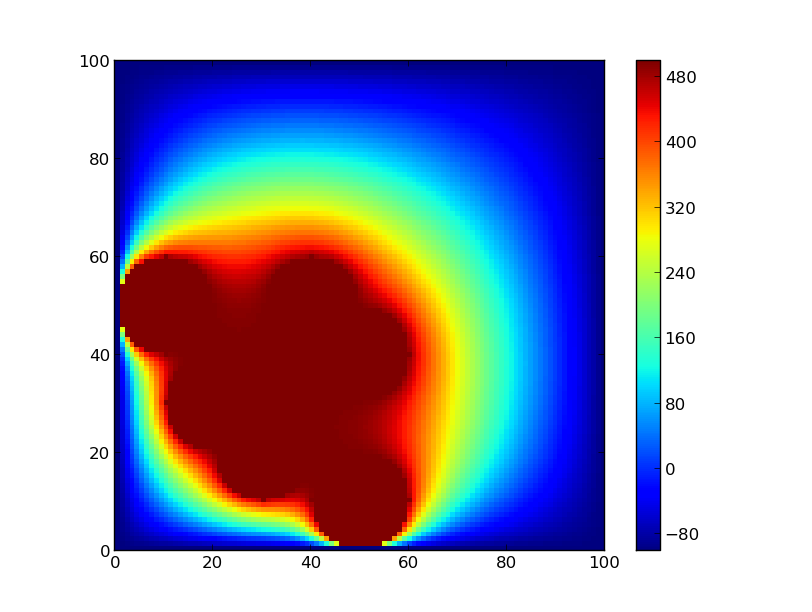
\includegraphics[width=110pt]{img/Parabrisas1-1.png} 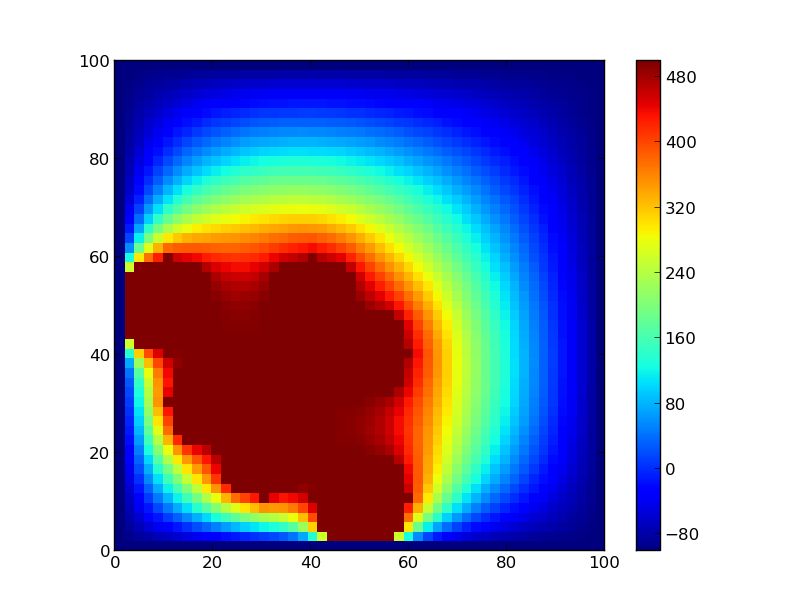
\includegraphics[width=110pt]{img/Parabrisas1-2.png} 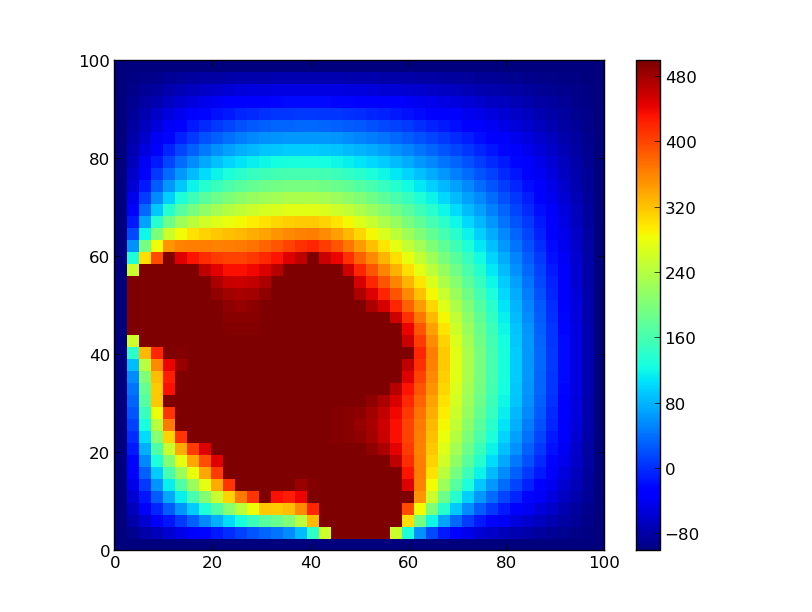
\includegraphics[width=110pt]{img/Parabrisas1-2,5.png} \newline 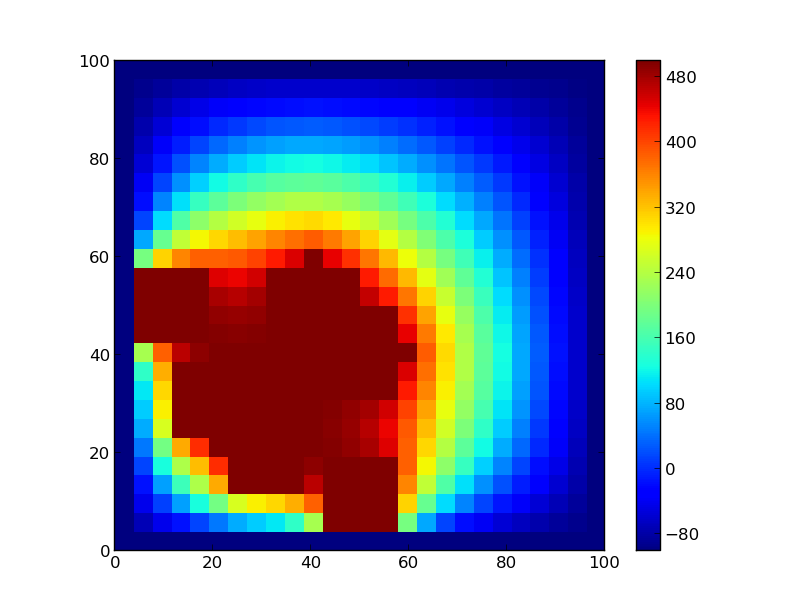
\includegraphics[width=110pt]{img/Parabrisas1-4.png} 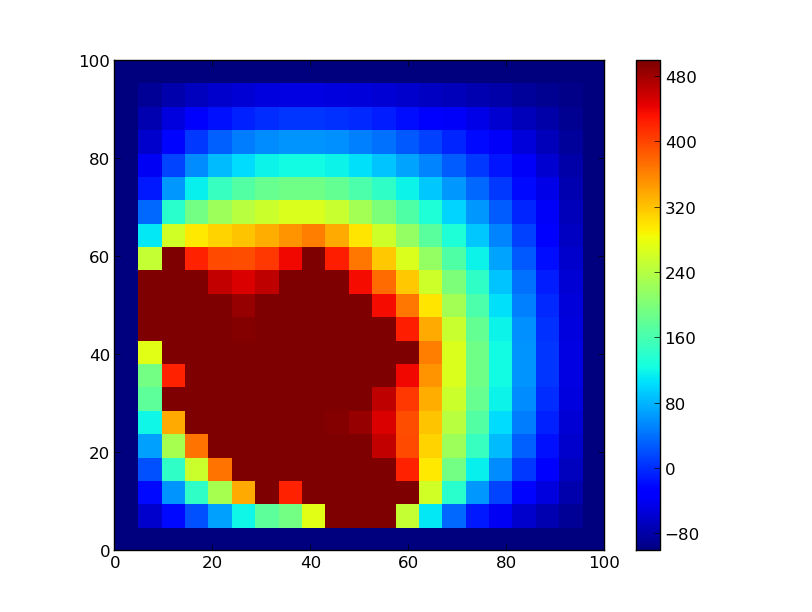
\includegraphics[width=110pt]{img/Parabrisas1-5.png} 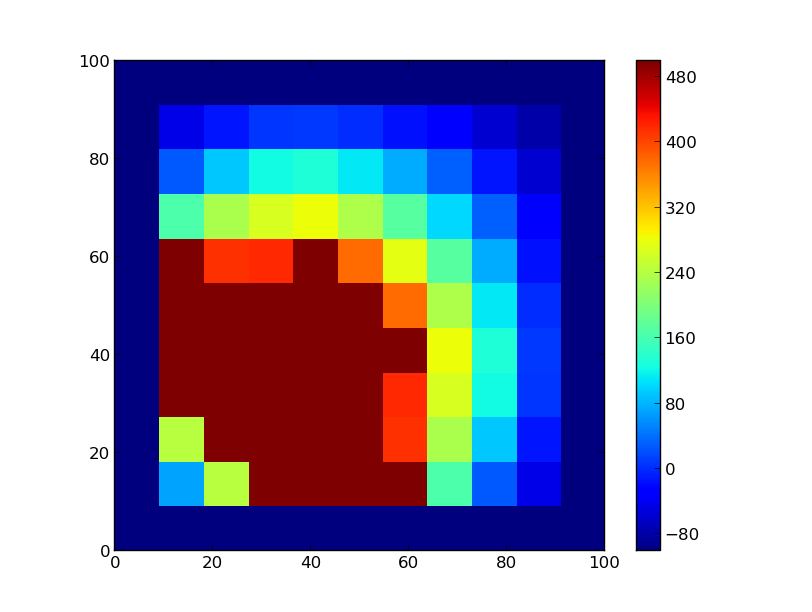
\includegraphics[width=110pt]{img/Parabrisas1-10.png} \newline
test2 \newline
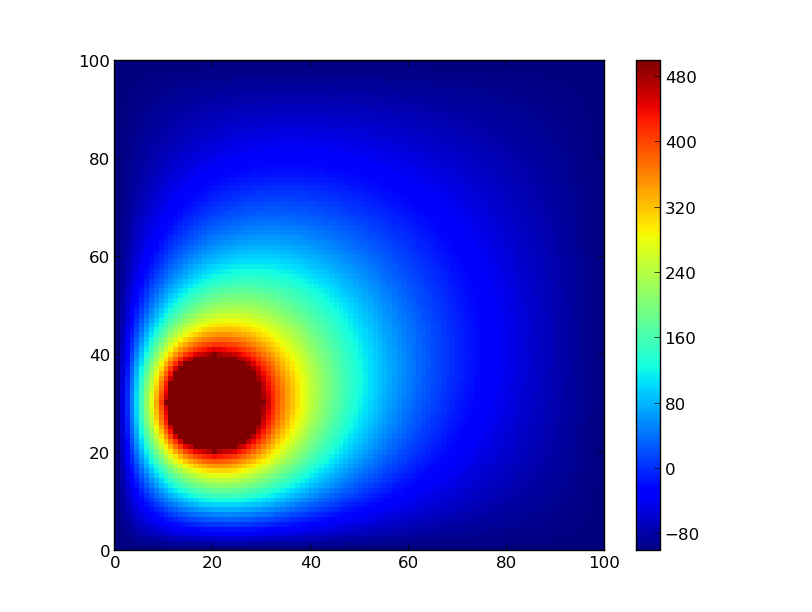
\includegraphics[width=110pt]{img/Parabrisas2-1.png} 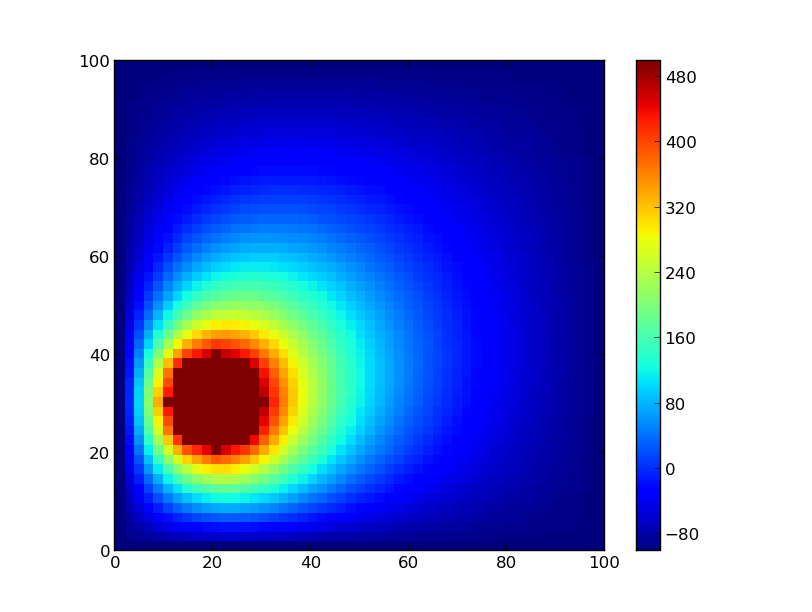
\includegraphics[width=110pt]{img/Parabrisas2-2.png} 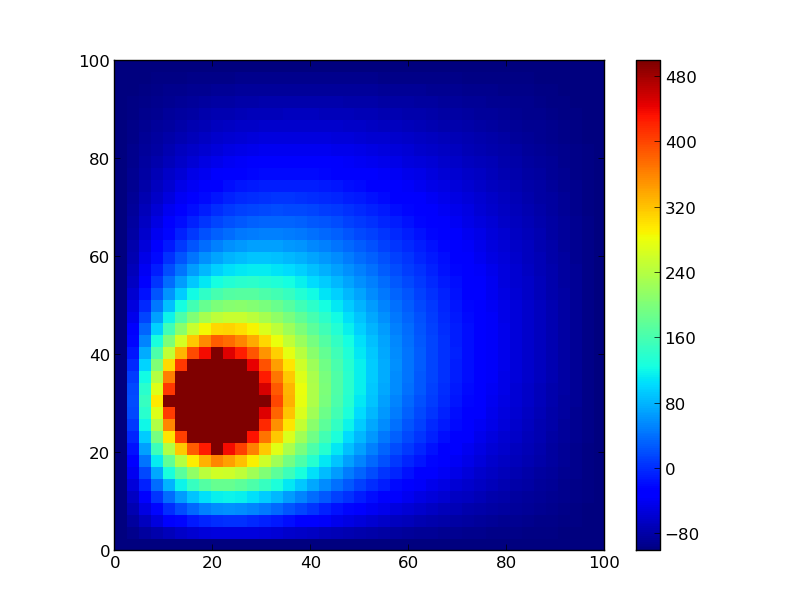
\includegraphics[width=110pt]{img/Parabrisas2-2,5.png} \newline 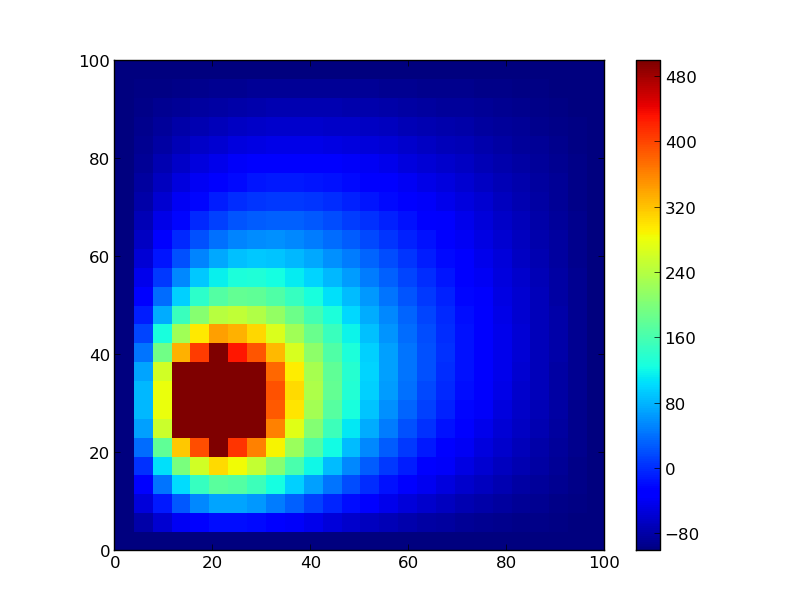
\includegraphics[width=110pt]{img/Parabrisas2-4.png} 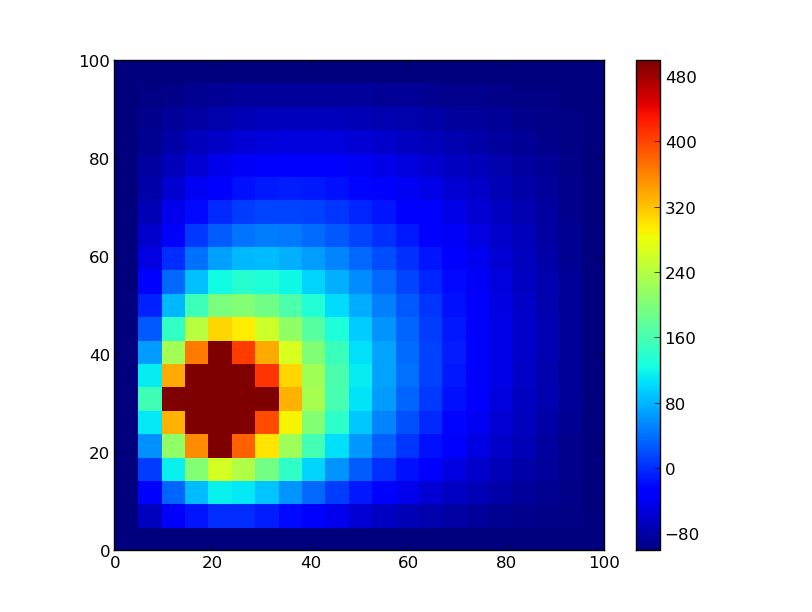
\includegraphics[width=110pt]{img/Parabrisas2-5.png} 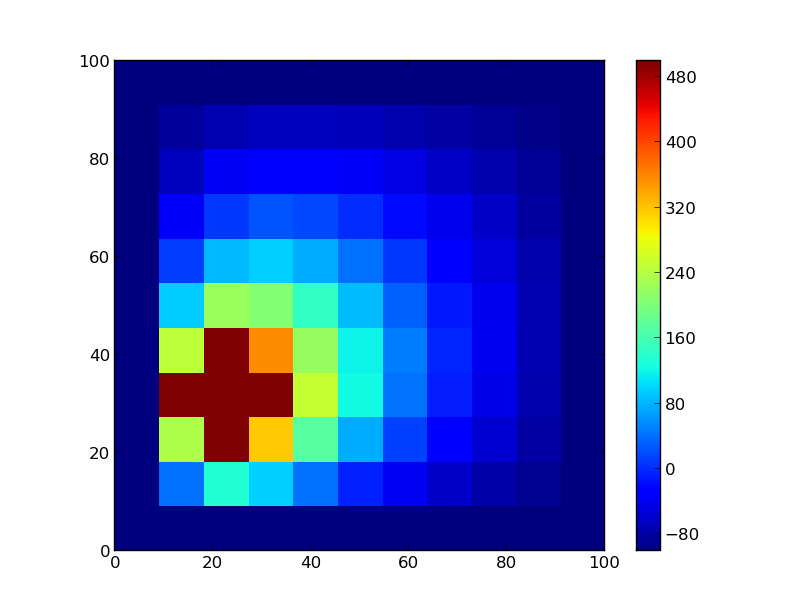
\includegraphics[width=110pt]{img/Parabrisas2-10.png} \newline
\newline
\newline
\newline
test3 \newline
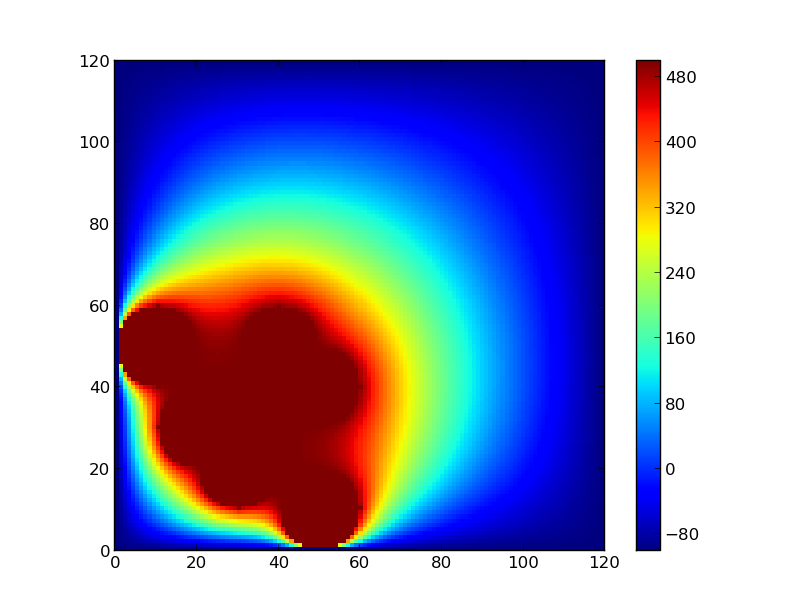
\includegraphics[width=110pt]{img/Parabrisas3-1.png} 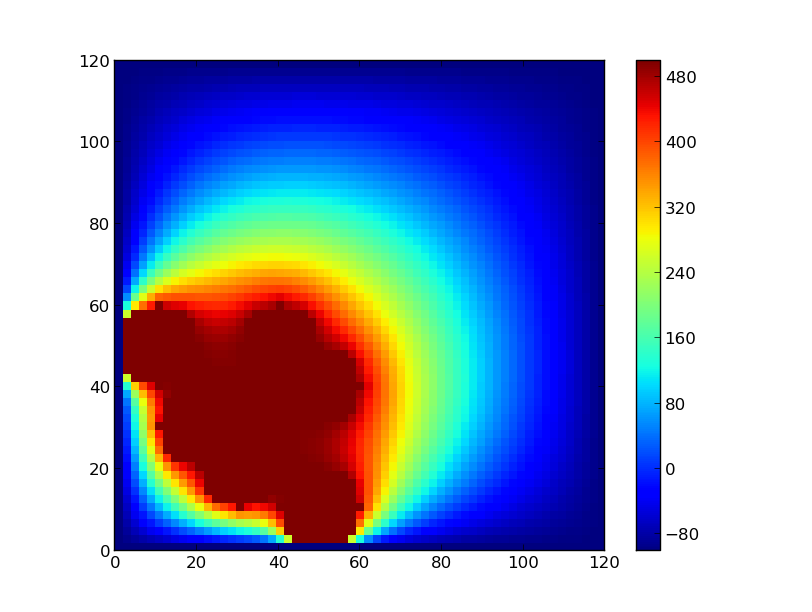
\includegraphics[width=110pt]{img/Parabrisas3-2.png} 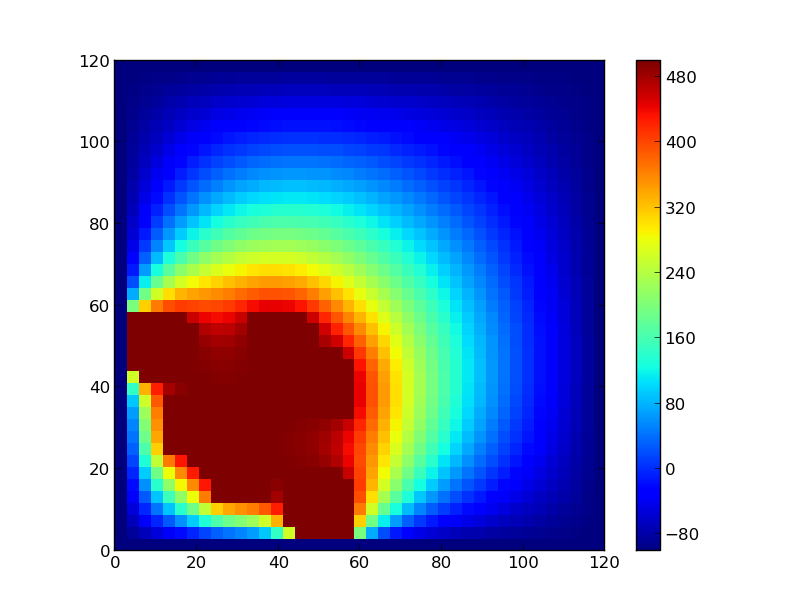
\includegraphics[width=110pt]{img/Parabrisas3-3.png} \newline 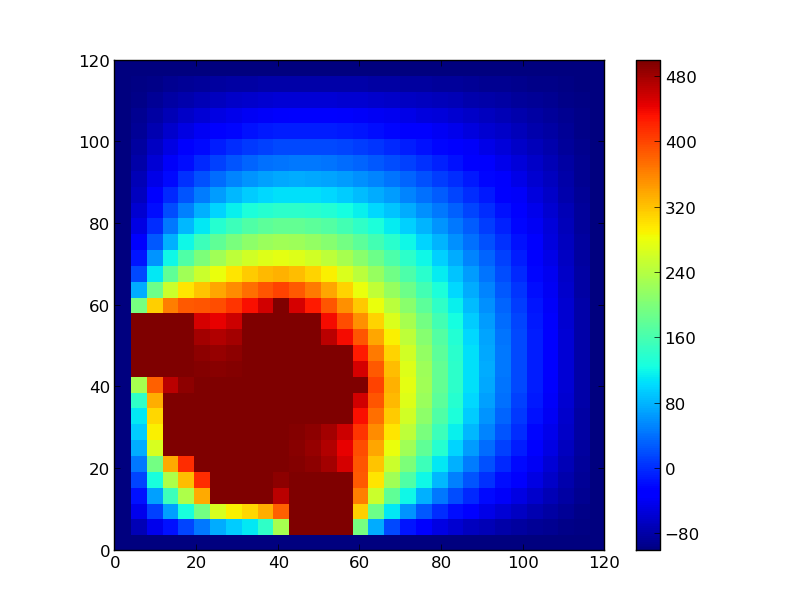
\includegraphics[width=110pt]{img/Parabrisas3-4.png} 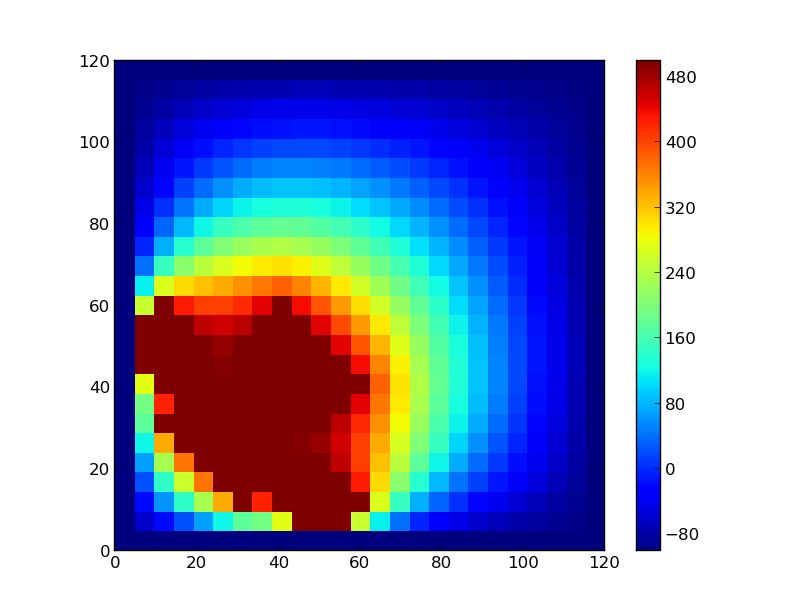
\includegraphics[width=110pt]{img/Parabrisas3-5.png} 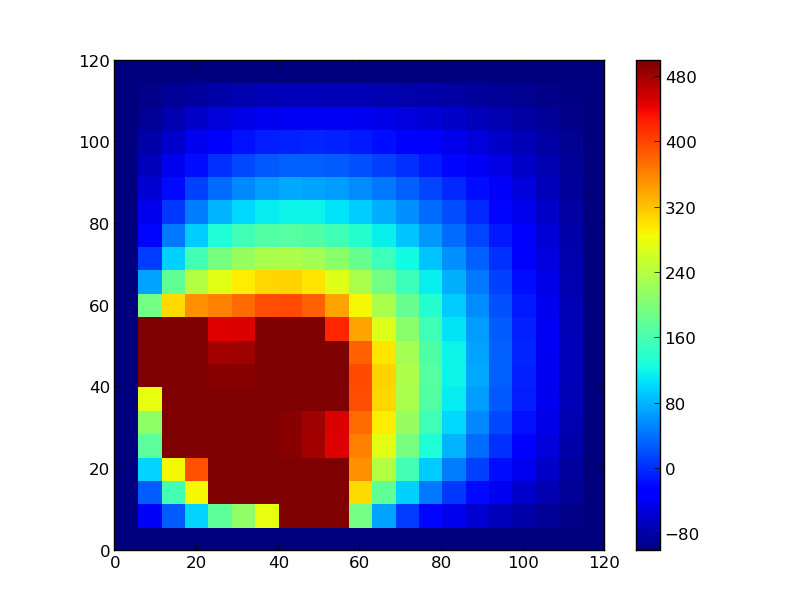
\includegraphics[width=110pt]{img/Parabrisas3-6.png} \newline
test4 \newline
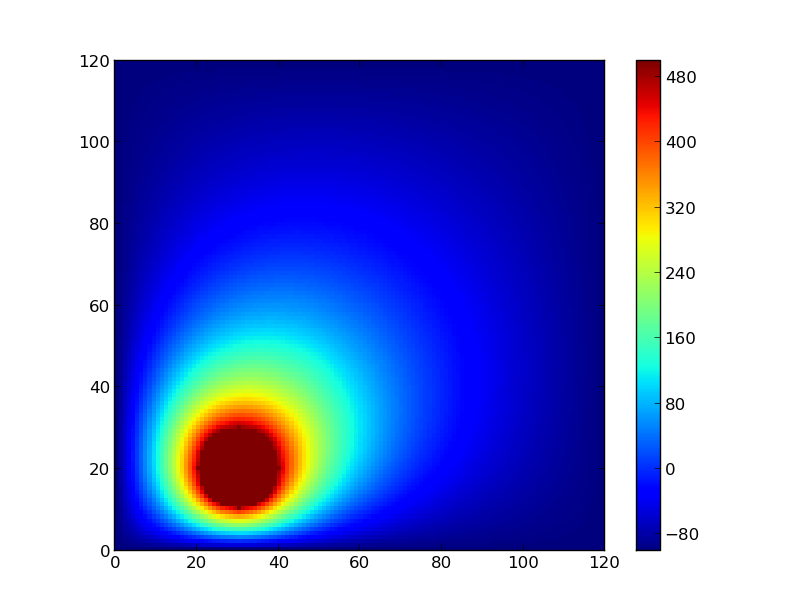
\includegraphics[width=110pt]{img/Parabrisas4-1.png} 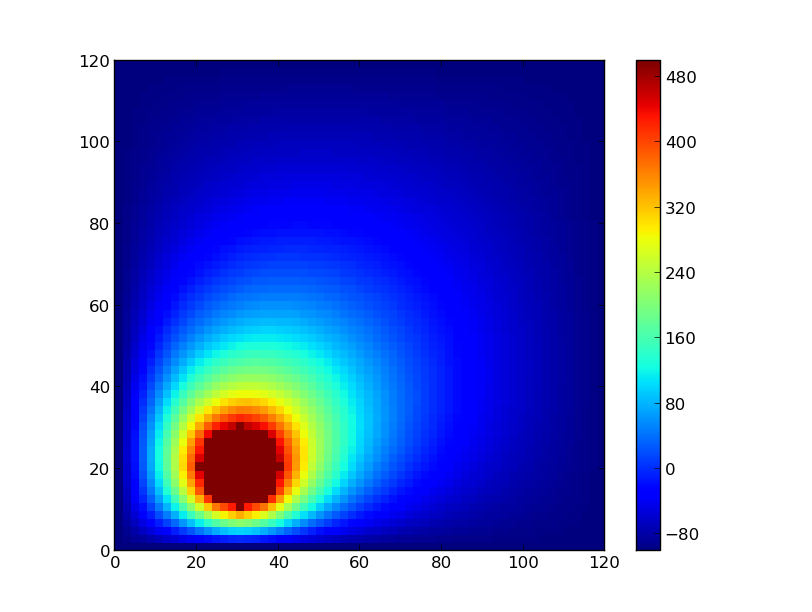
\includegraphics[width=110pt]{img/Parabrisas4-2.png} 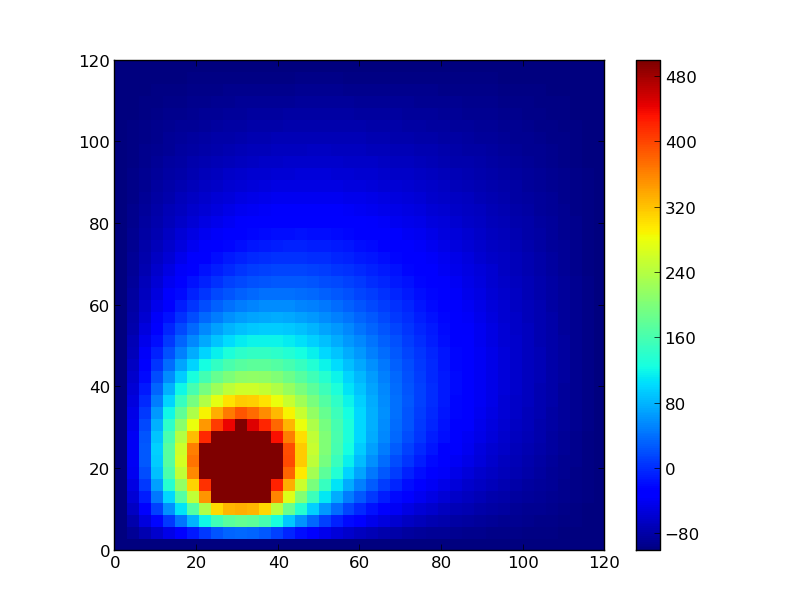
\includegraphics[width=110pt]{img/Parabrisas4-3.png} \newline 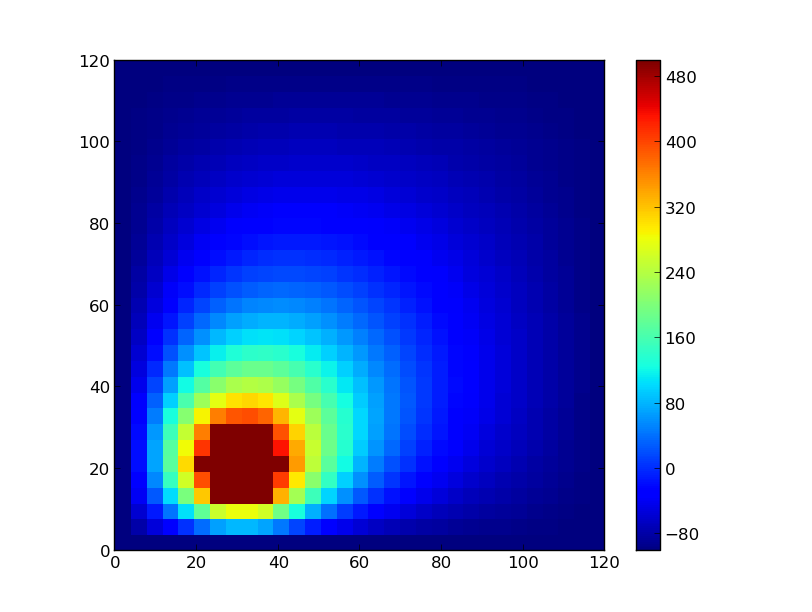
\includegraphics[width=110pt]{img/Parabrisas4-4.png} 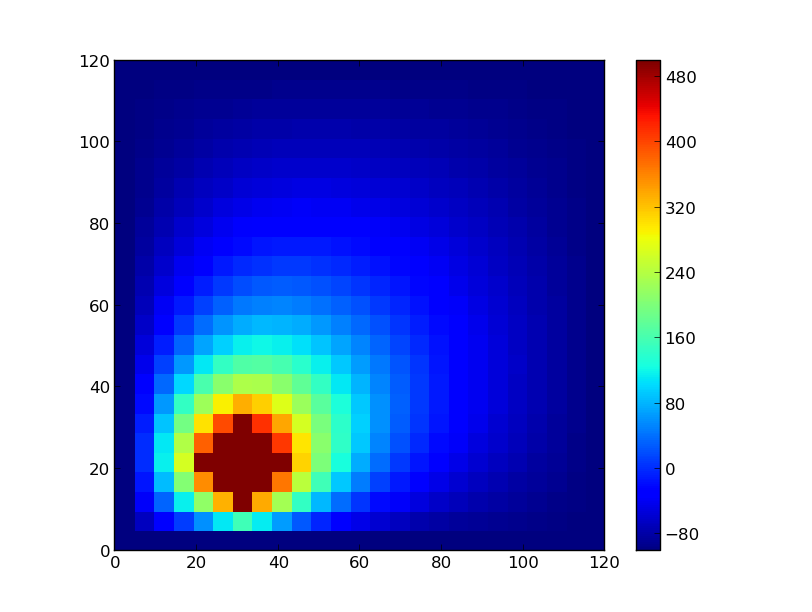
\includegraphics[width=110pt]{img/Parabrisas4-5.png} 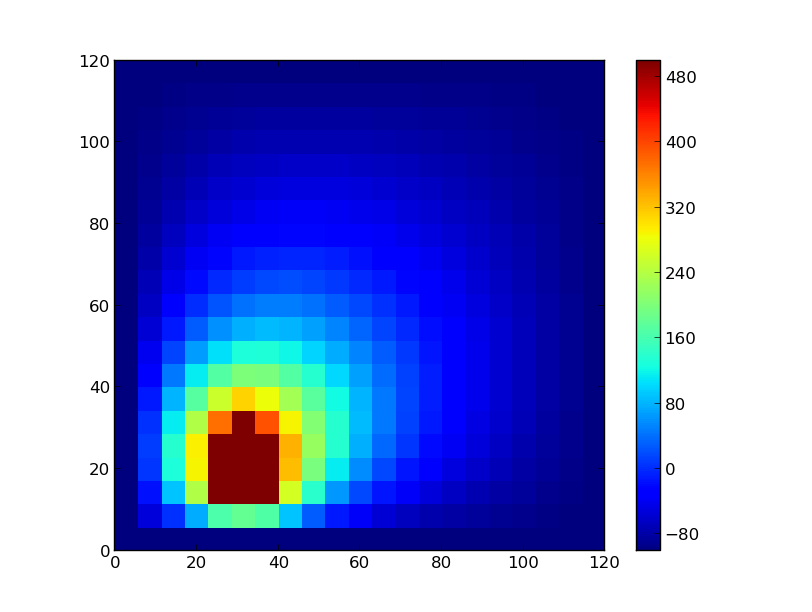
\includegraphics[width=110pt]{img/Parabrisas4-6.png} \newline

A continuación graficamos el tiempo de ejecución según la granularidad. En cada test difereciamos el método de elimiación gaussiana común y banda. Las mediciones las efectuamos anteponiendo el comando 'time' en la ejecución. Realizar varias mediciones producía una diferencia de hasta 0.5s, por lo tanto hicimos un promedio de varias ejecuciones; sin embargo, no se puede garantizar que los resultados para los casos de mayor granularidad sean confiables. Notar que la escala es logarítmica:

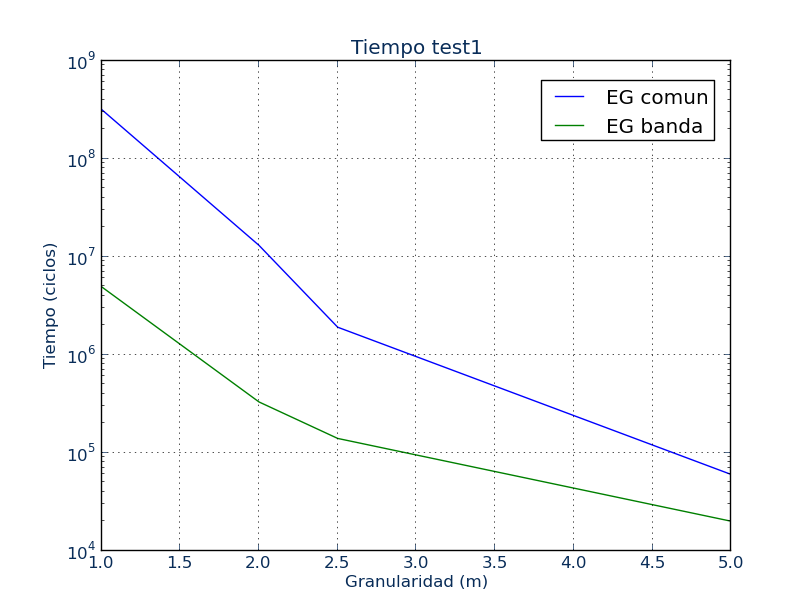
\includegraphics[width=180pt]{img/tiempo1.png}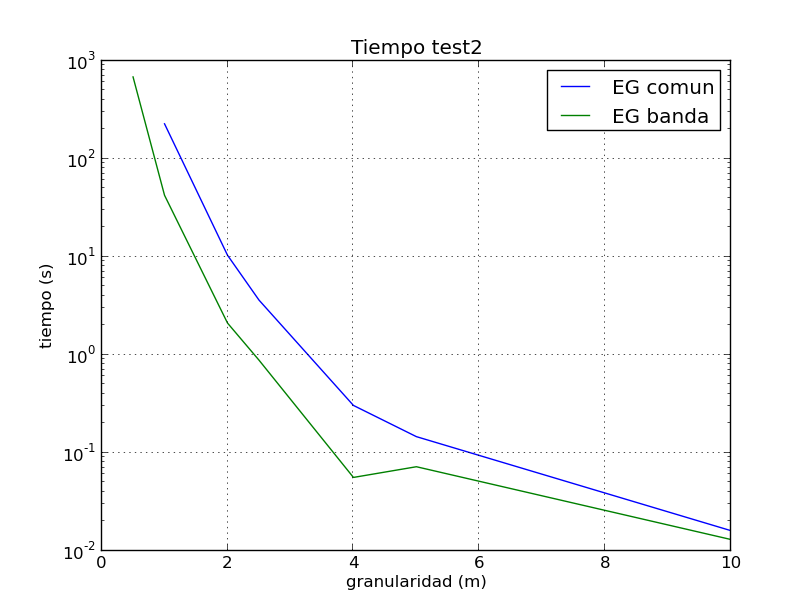
\includegraphics[width=180pt]{img/tiempo2.png} \newline
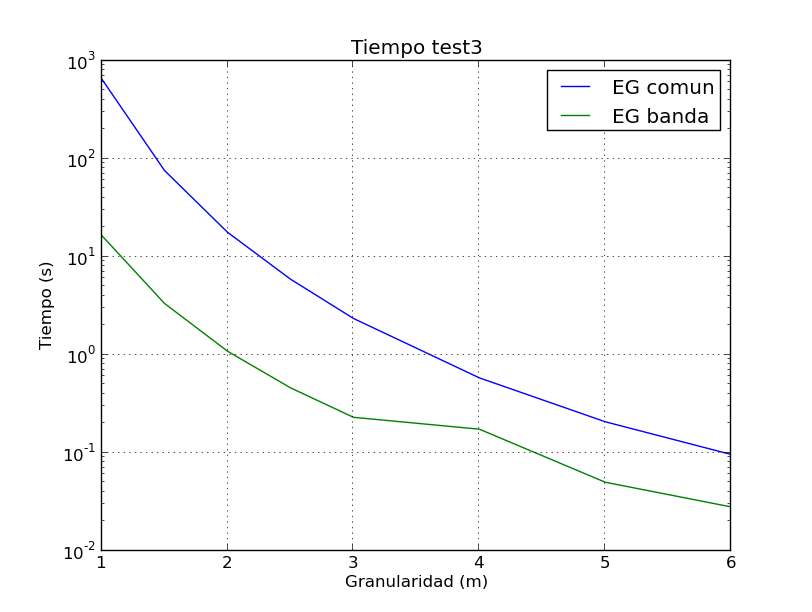
\includegraphics[width=180pt]{img/tiempo3.png}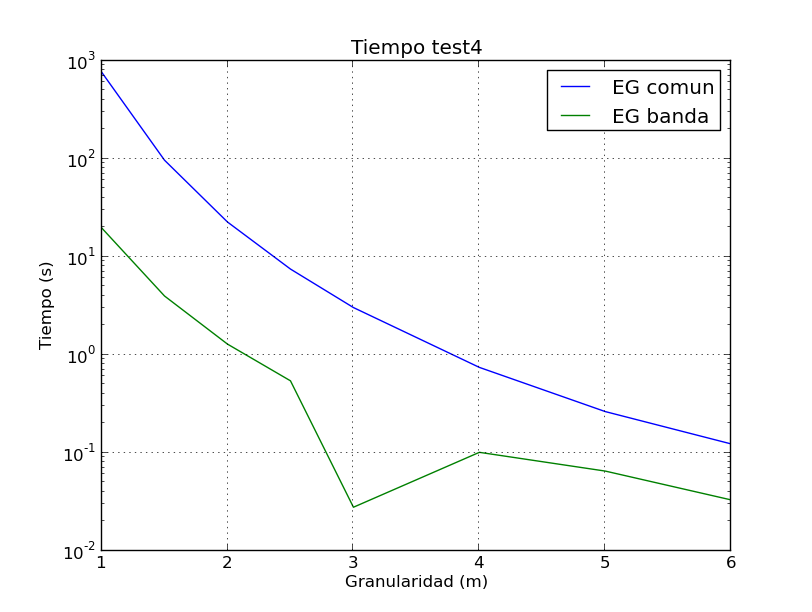
\includegraphics[width=180pt]{img/tiempo4.png} 

Lo que sigue es la temperatura del punto medio según la granularidad. Si $a/h$ o $l/h$ no es divisible por 2, entonces no hay una celda que se corresponda con el punto crítico. Una posibilidad para calcular su temperatura es, entonces, hacer un promedio de los cuatro puntos que lo rodean.

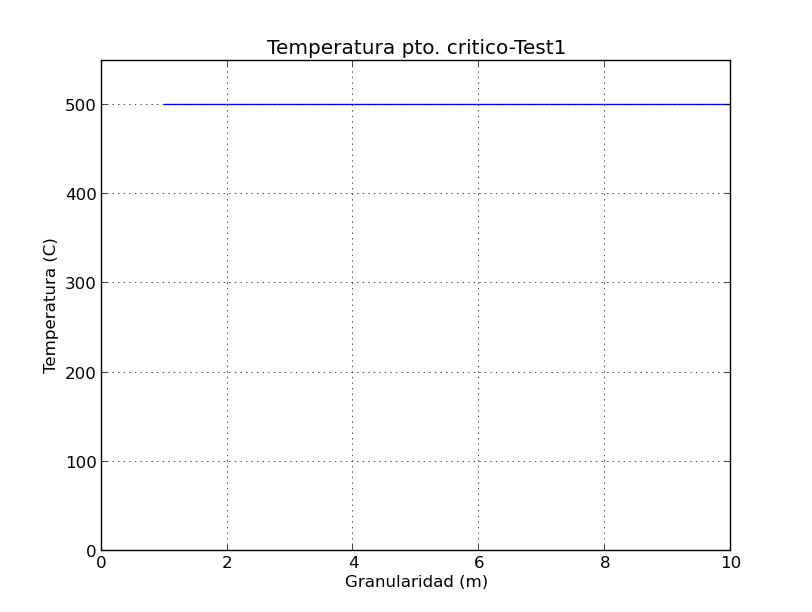
\includegraphics[width=180pt]{img/temp1.png}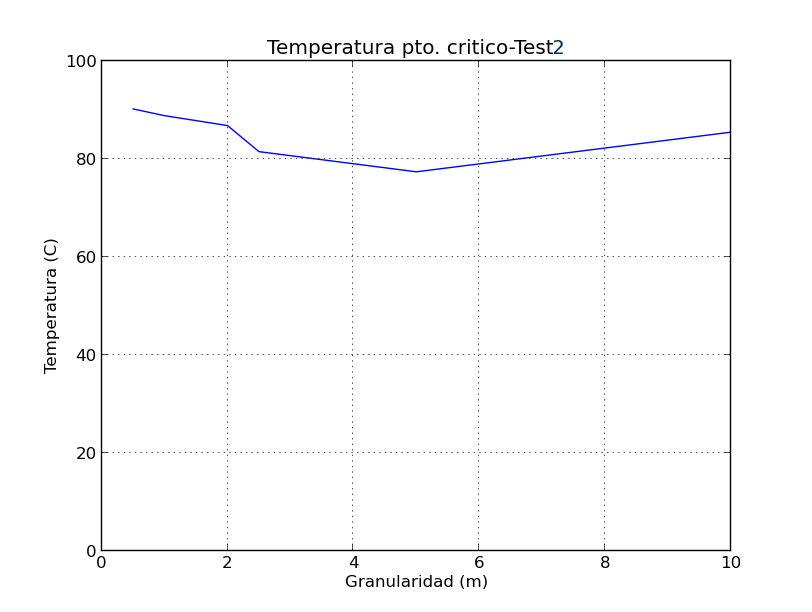
\includegraphics[width=180pt]{img/temp2.png} \newline
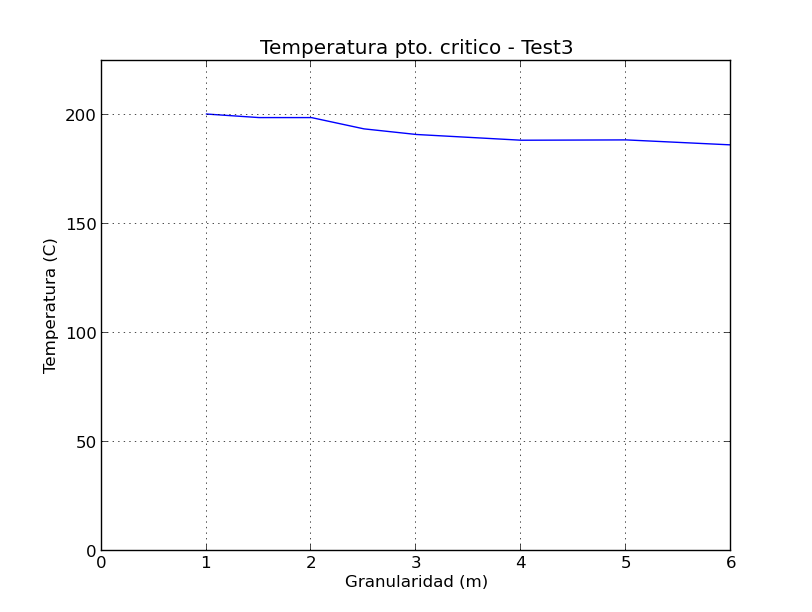
\includegraphics[width=180pt]{img/temp3.png}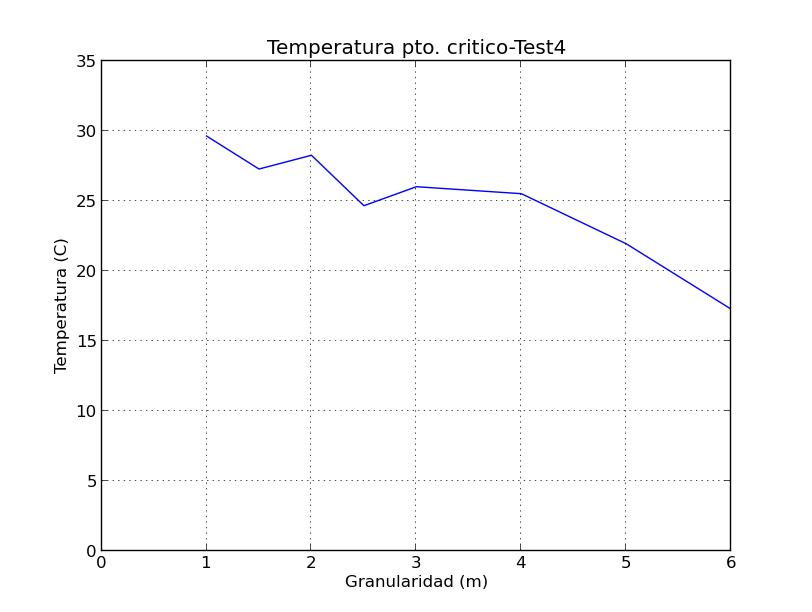
\includegraphics[width=180pt]{img/temp4.png}

Para el algoritmo de eliminación de sanguijuelas tomamos los tests 1 y 3, fijamos la granularidad en 2 y agregamos más sanguijuelas, de forma que el algoritmo tuviera que repetirse un número mayor de veces. \\
  \begin{tabular}{ l|l l l l l l}
  test & ancho & largo & h & radio & temp & $\#$sang \\
  \hline
  test1 & 100 & 100 & 2 & 10 & 500 & 15 \\
  test3 & 120 & 120 & 2 & 10 & 500 & 15 
\end{tabular} 

%graficar
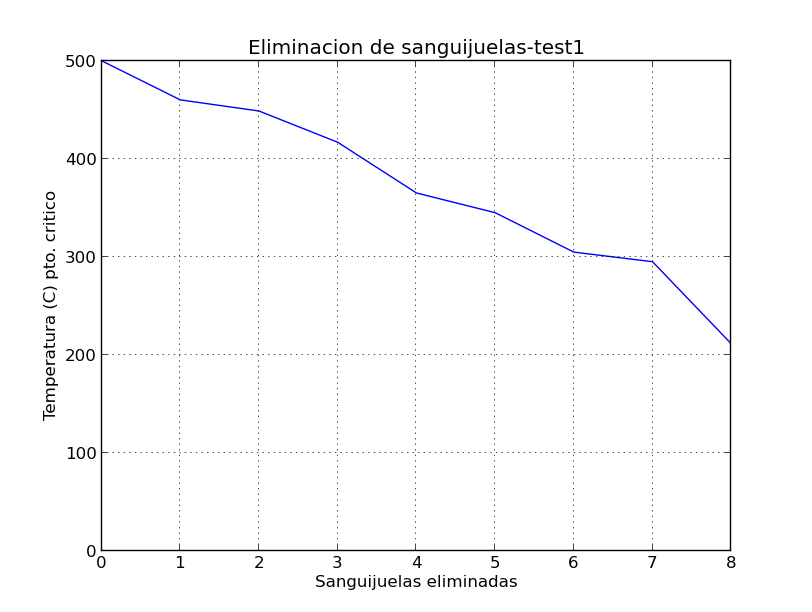
\includegraphics[width=300pt]{img/elim1.png} 

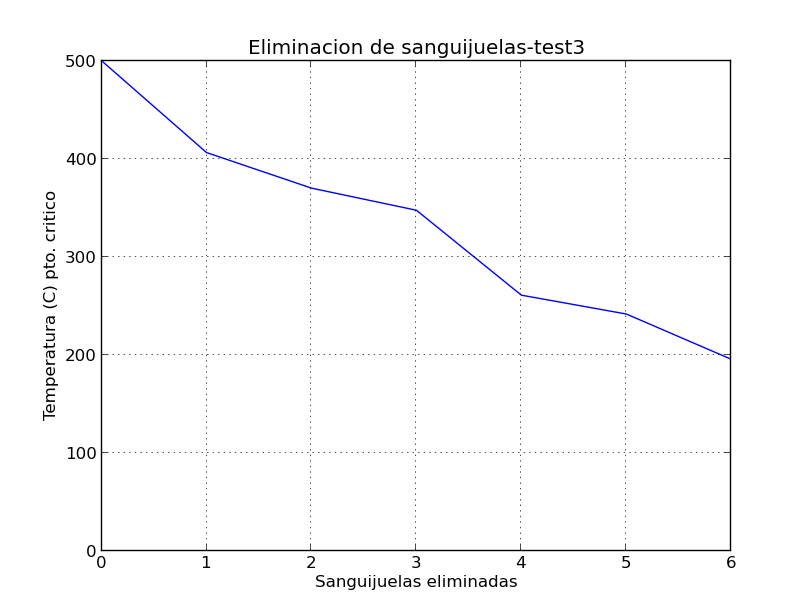
\includegraphics[width=300pt]{img/elim3.png} 

En cuanto al tiempo de ejecución, obtuvimos estos resultados que presentamos junto a los del test correspondiente, sin eliminación de sanguijuelas: \newline
\begin{tabular}{ l |l l l l}
  test & tiempo sin elim & tiempo con elim & $\#$ elim & $\frac{\text{tiempo con elim}}{\text{tiempo sin elim}}$\\
  \hline
  test1 & 1,413 & 8,361 & 8 & 5,91\\
  test3 & 3.159 & 13.347 & 6 & 4,22
\end{tabular} 


\newpage

\section{Discusi\'{o}n}
\label{sec:discusion}

Llamaremos $l$ al largo de la matriz parabrisas y $a$ a su ancho. 

Teniendo en cuenta que la matriz cuadrada es de $(l \times a) \times (l \times a)$ y que la matriz banda solo debe conservar $(l \times a) \times (2 \times a + 1)$ valores, la matriz banda ocupa menos memoria cuando $l > 2$. La diferencia escala con $l$. En el caso asintótico, ocupa $O(l^2 a^2)$ la matriz cuadrada y $O(l a^2)$ la matriz banda.

Como se puede ver en los gráficos de tiempo de ejecución, el algoritmo de eliminación gaussiana banda fue más eficiente que el común. El algoritmo banda tardó alrededor de $3l$ veces menos que el común en el test 1, algo que está en línea con lo que se esperaba. En los otros tests tardó más que eso, además de escalar la proporción más que $l$, por lo que podemos decir que la aproximación no fue muy buena.

La cantidad de sanguijuelas afectó al tiempo total de ejecución. En algunos casos lo aumentó y en otros lo redujo. Si bien al analizar el orden de complejidad en peor caso parecería que solo debería aumentarlo, hay que tener en cuenta que agregar una sanguijuela implica cambiar algunos valores de la matriz de 1/4 a 0. Esto reduce el tiempo de triangulación, que es el que domina la función.

Como esperábamos, reducir la granularidad aumentó el tiempo de ejecución. Se puede ver que una reducción de la granularidad del 50$\%$ llevó a un aumento del tiempo de ejecución del orden de $2^4$ en la matriz banda y hasta $2^5$ en la matriz común, aproximadamente; es decir, la mitad de lo esperado:\newline

Matriz banda \newline

\begin{tabular}{ l|l l l}
  test & h=1 & h=2 & $\frac{h=2}{h=1}$ \\
  \hline
  test1 & 42,007 & 2,006 & 15,272 \\
  test2 & 13,073 & 0,856 & 20,94 \\
  test3 & 69,18 & 4,427 & 15,62 \\
  test4 & 27,926 & 1,807 & 15,45 \\
\end{tabular} \newline \newline

Matriz común \newline

\begin{tabular}{ l|l l l}
  test & h=1 & h=2 & $\frac{h=2}{h=1}$ \\
  \hline
  test1 & 318,481 & 10,432 & 30,52 \\
  test2 & 431,00 & 4,380 & 32,40 \\
  test3 & 596,97 & 32,195 & 18,54 \\
  test4 & 711,23 & 27,969 & 25,42 \\
\end{tabular} \newline \newline

Sin embargo, se dieron casos anómalos en los tests 1 y 3, donde la curva resultante no fue decreciente, pero no sabemos a qué pueden deberse.

Reducir la granularidad llevó a resultados más exactos, como se puede ver en los mapas de temperatura. Con los gráficos de temperatura del punto crítico podemos ver que el valor de ese punto parece ir tendiendo hacia un determinado límite; si pudiéramos tomar un límite con granularidad tendiente a 0 entonces encontraríamos el valor del punto crítico en el caso continuo, en otras palabras, cuanta más precisa la granularidad, obtendremos un resultado más confiable y cercano al real.

En cuanto al algoritmo de eliminación, se pude ver que cada sanguijuela eliminada redujo la temperatura del punto crítico. Esto no garantiza que el algoritmo sea óptimo, ya que es evidente que si hubiera dos sanguijuelas en el mismo punto, esto no se daría. Pero dejando ese caso a un lado, podemos decir que el algortimo es bueno, ya que no desperdicia disparos en sanguijuelas que no afectan la temperatura del punto crítico.

En cuanto al tiempo de ejecución de este algoritmo, no coincide exactamente con el producto de la cantidad de sanguijuelas y el tiempo que se tarda en volver a calcular el sistema, si bien se aproxima. Esto se debe a que, como ya se dijo, recalcular el sistema con menos sanguijuelas no necesariamente cuesta lo mismo.

El cálculo de qué sanguijuela eliminar podría optimizarse si guardáramos un vector con la distancia al centro de cada sanguijuela, de forma que no habría que volver a calcular la de todas cada vez que se busca una a eliminar. Esta solución, sin embargo, ocuparía más espacio de memoria y no tendría un gran impacto en el tiempo total.


\newpage

\section{Conclusiones}
\label{sec:conclusiones}

Podemos, al final de nuestro trabajo, sacar varias conclusiones respecto al enfoque que le dimos a este problema (y el que suponemos que era esperado que le diéramos).

Primero, si se aumenta la granularidad, se pierde exactitud. Como consecuencia, el valor del punto crítico puede alejarse considerablemente del real, de forma que podría ser mayor a 235 cuando el real no lo es. Además, si el diámetro de las sanguijuelas es menor a la granularidad, una sanguijuela podría no cubrir ningún punto de la grilla, quedando el mapa de temperaturas como si ésta no estuviera, dando como resultado una temperatura menor en el punto crítico a la real. Es decir que es conveniente elegir una granularidad menor al diámetro de las sanguijuelas. Sin embargo, esto no siempre es posible, ya que el radio podría ser 0.

Teniendo esto en cuenta, junto al impacto de la granularidad en el tiempo de ejecución, podemos decir que obtuvimos los mejores resultados con granularidad alrededor de 1/50 del lado, con un parabrisas cuadrado. Por supuesto, hay factores que modifican esto, como cuán precisa debe ser la medición del valor del punto crítico.

Podemos sacar otras conclusiones al ver las diferencias que surgen de implementar una matriz como una banda o como una común.

Principalmente se puede ver la importancia que tiene el no guardar más datos de los necesarios (o de guardarlos de manera inteligente) para cubrir todas las funciones esperadas de nuestra estructura de manera satisfactoria, ya que es evidente que si bien ambas implementaciones cumplen con lo necesario para considerarse correctas, la eficiencia, tanto a nivel temporal como espacial, de la matriz banda sobrepasa por mucho a aquella de la matriz común.
Habiendo dicho esto, uno podría pensar que la matriz banda sería deseable por sobre la común en todos los casos, pero podemos hacernos la pregunta de si no hay algo que estemos perdiendo al obtener esta mayor eficiencia.  Salta entonces a la vista que la matriz banda se diferencia de la común en que está mucho más especializada, es decir que al aprovechar el hecho de que trabaja con una matriz con forma de banda, al asumir que los puntos alejados del centro a partir de una determinada distancia valen 0 estamos justamente reduciendo la cantidad de casos a los que la matriz banda es aplicable. La matriz banda trabaja mejor con todos los casos que puede, pero es aplicable a menos casos, mientras que la común cambia velocidad y memoria por una versatilidad mucho mayor.
En otras palabras, si quisiéramos usar la banda para alguna otra utilidad, distinta del trabajo que se nos pidió en este enunciado, tendríamos primero que comprobar si es aplicable a nuestros experimentos, mientras que con la común ya directamente no habría requisitos para representar en forma de matriz lo que sea que necesitemos.
Luego de haber sacado conclusiones de comparar nuestras implementaciones en términos de versatilidad, velocidad y tiempo, queda también ver qué podemos sacar de la comparación entre complejidad de implementaciones; sin embargo no encontramos mucha diferencia entre nuestra implementación de matriz banda y de común, ya que nos limitamos a reducir el ancho de la matriz efectiva que guardábamos, incluso comparten funciones (con ligeras variaciones).


\newpage
\section{Apéndice A}
\label{sec:ApA}


\documentclass[11pt, a4paper]{article}
\usepackage{a4wide}
\usepackage{amsmath}
\usepackage{amsfonts}
\usepackage{graphicx}
\usepackage{color}
\usepackage{todonotes}
%\usepackage[ruled,vlined]{algorithm2e}

\parskip = 11pt

\newcommand{\real}{\mathbb{R}}
\newcommand{\nat}{\mathbb{N}}

\newcommand{\atacante}{sanguijuela}
\newcommand{\capitan}{Capit\'an Guybrush Threepwood}
\newcommand{\objeto}{parabrisas}
\newcommand{\nave}{El Pepino Marino}

\newcommand{\revJ}[1]{{\color{red} #1}}

\begin{document}


\begin{centering}
\large\bf Laboratorio de M\'etodos Num\'ericos - Segundo Cuatrimestre 2014 \\
\large\bf Trabajo Pr\'actico N\'umero 1: \emph{``No creo que a \'el le gustara eso''}\\
\end{centering}


\vskip 0.5 cm
\hrule
\vskip 0.1 cm

{\noindent \bf Introducci\'on}

El afamado \capitan\ se encuentra nuevamente en problemas. El
\objeto\ de su nave \nave\ est\'a siendo atacado simult\'aneamente por varios
dispositivos hostiles vulgarmente conocidos como \emph{\atacante s
mutantes}. Estos artefactos se adhieren a los \objeto\ de las naves y
llevan a cabo su ataque aplicando altas temperaturas sobre la superficie, con
el objetivo de debilitar la resistencia del mismo y permitir as\'\i \
un ataque m\'as mort\'\i fero. Cada \atacante\ consta de una \emph{sopapa
de ataque} circular, que se adhiere al \objeto\ y aplica una temperatura
constante sobre todos los puntos del \objeto\ en contacto con la sopapa.

Para con\-tra\-rres\-tar estas acciones hostiles, el \capitan\ 
solamente cuenta con el sistema de refrigeraci\'on de la nave, que puede
aplicar una temperatura constante de -100${}^o$C a los bordes del \objeto.
El manual del usuario de la nave dice que si el punto central del \objeto\ 
alcanza una temperatura de 235${}^o$C, el \objeto\ no resiste la temperatura
y se destruye. Llamamos a este punto el \emph{punto cr\'\i tico} del
\objeto.

En caso de que el sistema de refrigeraci\'on no sea suficiente para salvar
el punto cr\'\i tico, nues\-tro \capitan\ tiene todav\'\i a una posibilidad
adicional: puede des\-tru\-ir algunas de las \atacante s, pero debe eliminar la
menor cantidad posible de \atacante s dado que cada eliminaci\'on consume
energ\'\i a que puede ser vital para la concreci\'on de la misi\'on.
La situaci\'on es desesperante, y nuestro h\'eroe debe tomar una r\'apida
determinaci\'on: debe decidir qu\'e \atacante s eliminar de modo tal que el
\objeto\ resista hasta alcanzar la base m\'as cercana.

{\noindent \bf El modelo}

Suponemos que el \objeto\ es una placa rectangular de $a$ metros de ancho y $b$ metros de altura. Llamemos $T(x,y)$ a la temperatura en el punto dado por las coordenadas $(x,y)$. En el estado estacionario, esta temperatura satisface la ecuaci\'on del calor:

\begin{equation}\label{eq:calor}
\frac{\partial^2T(x,y)}{\partial x^{2}}+\frac{\partial^2 T(x,y)}{\partial y^{2}} = 0.
\end{equation}

\noindent La temperatura constante en los bordes queda definida por la siguiente ecuaci\'on:
\begin{equation}
T(x,y) = -100^o\textrm{C}~~~~~\textrm{si } x = 0,a \textrm{ \'o } y = 0,b.
\label{eq:borde}
\end{equation}

\noindent De forma an\'aloga es posible fijar la temperatura en aquellos puntos cubiertos por una \atacante, considerando $T_s$ a la temperatura ejercida por las mismas.

El problema en derivadas parciales dado por la primera ecuaci\'on con las condiciones de contorno presentadas recientemente, permite encontrar la funci\'on $T$ de temperatura en el \objeto, en funci\'on de los datos mencionados en esta secci\'on.

%(x_j,y_i) = (ib/n,ja/m)
Para estimar la temperatura computacionalmente, con\-si\-de\-ra\-mos la siguiente discretizaci\'on del \objeto: sea $h \in \mathbb{R}$ la granularidad de la discretizaci\'on, de forma tal que $a = m\times h$ y $b = n \times h$, con $n,m \in \mathbb{N}$, obteniendo as\'i una grilla de $(n+1)\times(m+1)$ puntos. Luego, para $i=0,1,\dots,n$ y $j=0,1,\dots,m$, llamemos $t_{ij} = T(x_j,y_i)$ al valor (desconocido) de la funci\'on $T$ en el punto $(x_j, y_i) = (ih, jh)$, donde el punto $(0,0)$ se corresponde con el extremo inferior izquierdo del \objeto.
La aproximaci\'on por \emph{diferencias finitas} de la ecuaci\'on del calor afirma que:
\begin{equation}
t_{ij} \ =\ \frac{ t_{i-1,j} + t_{i+1,j} + t_{i,j-1} + t_{i,j+1}}{4}.\label{eq:calordd}
\end{equation}

Es decir, la temperatura de cada punto de la grilla debe ser igual al promedio de las tem\-pe\-ra\-tu\-ras de sus puntos vecinos en la grilla. Adicionalmente, conocemos la temperatura en los bordes, y los datos del problema permiten conocer la temperatura en los puntos que est\'an en contacto con las \atacante s.

{\noindent \bf Enunciado}

Se debe implementar un programa en \verb+C+ o \verb-C++- que tome como entrada los par\'ametros del problema ($a$, $b$, $n$, $m$, $r$, $T_s$ y las posiciones de las \atacante s) que calcule la temperatura en el \objeto\ utilizando el modelo propuesto en la secci\'on anterior y que determine a qu\'e \atacante s dispararle con el fin de evitar que se destruya el \objeto. El m\'etodo para determinar las \atacante s que ser\'an destru\'idas queda a criterio del grupo, y puede ser exacto o heur\'istico.

Para resolver este problema, se deber\'a formular un sistema de ecuaciones lineales que permita calcular la temperatura en todos los puntos de la grilla que discretiza el \objeto, e implementar el m\'etodo de Eliminaci\'on Gaussiana (EG) para resolver este sistema particular. Dependiendo de la granularidad utilizada en la discretizaci\'on, el sistema de ecuaciones resultante para este problema puede ser muy grande. Luego, es importante plantear el sistema de ecuaciones de forma tal que posea cierta estructura (i.e., una matriz banda), con el objetivo de explotar esta caracter\'istica tanto desde la \emph{complejidad espacial} como \emph{temporal} del algoritmo.

En funci\'on de la implementaci\'on, como m\'inimo se pide:
\begin{enumerate}
\item Representar la matriz del sistema utilizando como estructura de datos los tradicionales arreglos bi-dimensionales. Implementar el algoritmo cl\'asico de EG. \label{enum:EGcomun}
\item Representar la matriz del sistema aprovechando la estructura banda de la misma, haciendo hincapi\'e en la complejidad espacial.  Realizar las modificaciones necesarias al algoritmo de EG para que aproveche la estructura banda de la matriz. \label{enum:EGbanda}
\end{enumerate}

En funci\'on de la experimentaci\'on, como m\'inimo deben realizarse los siguientes experimentos:

\begin{itemize}
\item Considerar al menos dos instancias de prueba, generando discretizaciones variando la granularidad para cada una de ellas y comparando el valor de la temperatura en el punto cr\'itico. Se sugiere presentar gr\'aficos de temperatura para los mismos, ya sea utilizando las herramientas provistas por la c\'atedra o implementando sus propias herramientas de graficaci\'on. 
\item Analizar el tiempo de c\'omputo requerido en funci\'on de la granularidad de la discretizaci\'on, buscando un compromiso entre la calidad de la soluci\'on obtenida y el tiempo de c\'omputo requerido. Comparar los resultados obtenidos para las variantes propuestas en \ref{enum:EGcomun} y \ref{enum:EGbanda}. 
\item Estudiar el comportamiento del m\'etodo propuesto para la estimaci\'on de la temperatura en el punto cr\'itico y para la eliminaci\'on de \atacante s.
\end{itemize}

Finalmente, se deber\'a presentar un informe que incluya una descripci\'on detallada de los m\'etodos implementados y las decisiones tomadas, incluyendo las estructuras utilizadas para representar la matriz banda  y los experimentos realizados, junto con el correspondiente an\'alisis y siguiendo las pautas definidas en el archivo \verb+pautas.pdf+.

{\noindent \bf Programa y formato de archivos}

El programa debe tomar tres par\'ametros (y en ese orden): el archivo de entrada, el archivo de salida y el m\'etodo a ejecutar (0: EG com\'un, 1: EG banda).
El archivo de entrada contiene los datos del problema (tama\~no del
\objeto, ubicaci\'on, radio y temperatura de las \atacante s) desde un
archivo de texto con el siguiente formato:

\begin{verbatim}
      (a)  (b)  (h)  (r)  (t)  (k)
      (x1) (y1)
      (x2) (y2)
      ...
      (xk) (yk)
\end{verbatim}

En esta descripci\'on, $a\in\real_+$ y $b\in\real_+$ representan el ancho
y largo en metros del \objeto, respectivamente. De acuerdo con la descripci\'on
de la discretizaci\'on del \objeto, $h$ es la longitud de cada intervalo de discretizaci\'on,
obteniendo como resultado una grilla de $n+1\in\nat$ filas y $m+1\in\nat$ columnas.
Por su parte, $r\in\real_+$ representa el radio de las sopapas de ataque de las
\atacante s (en metros), $t\in\real$ es la temperatura de ataque de las sopapas,
y $k\in\nat$ es la cantidad de \atacante s. Finalmente, para $i=1,\dots,k$,
el par $(x_i,y_i)$ representa la ubicaci\'on de la $i$-\'esima sanguijuela en el
\objeto, suponiendo que el punto $(0,0)$  corresponde al extremo inferior
izquierdo del mismo.

El archivo de salida contendr\'a los valores de la temperatura en cada punto de la discretizaci\'on utilizando la informaci\'on original del problema (es decir, antes de aplicar el m\'etodo de remoci\'on de sanguijuelas), y ser\'a utilizado para realizar un testeo parcial de correctitud de la implementaci\'on. El formato del archivo de salida contendr\'a, una por l\'inea, el indicador de cada posici\'on de la grilla $i$, $j$ junto con el correspondiente valor de temperatura. A modo de ejemplo, a continuaci\'on se muestran c\'omo se reportan los valores de temperatura para las posiciones $(3,19)$, $(3,20)$, $(4,0)$ y $(4,1)$. 

\begin{verbatim}
      ...
      3   19  -92.90878
      3   20  -100.00000
      4   0   -100.00000
      4   1   60.03427
      ...
\end{verbatim}

El programa debe ser compilado, ejecutado y testeado utilizando los \emph{scripts} de \emph{python} que acompa\~nan este informe. Estos permiten ejecutar los tests provistos por la c\'atedra, incluyendo la evaluaci\'on de los resultados obtenidos e informando si los mismos son correctos o no. Es requisito que el c\'odigo entregado pase satisfactoriamente los casos de tests provistos para su posterior correcci\'on. Junto con los archivos podr\'an encontrar un archivo \texttt{README} que explica la utilizaci\'on de los mismos.

\vskip 0.5 cm
\hrule
\vskip 0.1 cm

{\bf Fecha de entrega} 
\begin{itemize}
\item \textsl{Formato electr\'onico:} Jueves 04 de Septiembre de 2014, \underline{hasta las 23:59 hs.}, enviando el trabajo
(\texttt{informe} + \texttt{c\'odigo}) a \texttt{metnum.lab@gmail.com}. El \texttt{asunto} del email debe comenzar con el texto \verb|[TP1]| seguido
de la lista de apellidos de los integrantes del grupo. Ejemplo: \texttt{[TP1] D\'iaz, Bianchi, Borghi}
\item \textsl{Formato f\'isico:} Viernes 05 de Septiembre de 2014, de 17:30 a 18:00 hs.
\end{itemize}


\end{document}


\newpage

\section{Referencias}
\label{sec:ref}

Apuntes de clase

R. Burden y J.D.Faires, Análisis numérico, International Thomson Editors, 1998

\end{document}